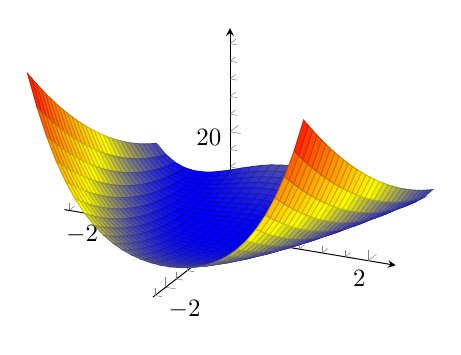
\begin{tikzpicture}
[
        scale=0.90,
        declare function = {
           % q(\x) = \x - 1;
            %Z(\x,\y) = sin(0.5* \x^2 - 0.25 * \y^2 + 3) * cos(2 * \x - \y); %* cos(2* \x + 1 - exp(\y)); %+ \x^2 + \y^2 + 1; %q(\x);
            Z(\x,\y) = (1-\x)^2 + 100(\y-\x^2)^2;
        }
    ]
    \begin{axis}
    [
    axis lines=center,
    enlargelimits,
    tick align=inside,
    domain=-2:2,
    samples=30, % this was 200, but I changed it to 20 because of my slow PC
    minor tick num=5,
    ]
    \addplot3 [surf] {Z(x,y)};
    \end{axis}
\end{tikzpicture}
